	\documentclass[twoside]{article}
\usepackage{../../estilo-ejercicios}

%--------------------------------------------------------
\begin{document}

\title{Relación 3}
\author{Javier Aguilar Martín}
\maketitle


\begin{ejercicio}{3.1}
Compute the chromatic number of the following graphs:

\begin{figure}[h!]
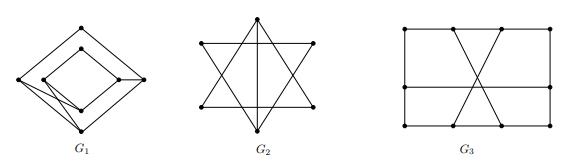
\includegraphics[scale=0.7]{grafos31}
\end{figure}
\end{ejercicio}
\begin{solucion}
$\chi(G_1)=3$: Si intentamos dar una 2-coloración, los dos vértices de abajo a la izquierda en el cuadrado exterior deben tener colores 1 y 2 respectivamente, con lo que los de abajo a la izquierda en el cuadrado interior deben tener esos colores en el mismo orden, y de ahí los vértices de arriba a la derecha del cuadrado interior deben tenerlos en orden opuesto. De aquí, el vértice más a la derecha del cuadrado externo debe tener el color 2, con lo que el vértice que queda libre tendría que tener el color 1, pero es adyacente al primero que coloreamos con color 1, así que necesitamos un tercer color. 

Como $G_2$ contiene $K_3$, $\chi(G_2)\geq 3$. Como además es tripartido tenemos la desigualdad opuesta, así que $\chi(G_2)=3$. 

$\chi(G_3)=2$: empezar dando colores 1 y 2 a los del medio y después ir completando. 
\end{solucion}

\newpage


\begin{ejercicio}{3.2}
Which of the following hold true?
\begin{enumerate}[a)]
\item For every $n ≥ 4$ there exists a planar graph $G$ with $n$ vertices and chromatic
number $χ(G) = 4$.
\item If $χ(G) ≤ 4$ then $G$ is planar.
\item There exists a graph $G$ with $χ(G) = 3$ and independence number 5.
\end{enumerate}
\end{ejercicio}
\begin{solucion}\
\begin{enumerate}[a)]
\item es cierto porque basta partir de $K_4$, que es planar, y añadir vértices aislados.
\item falso, $\chi(K_{3,3})=2$. 
\item cierto, $K_{5,5,5}$.  
\end{enumerate}

\end{solucion}

\newpage

\begin{ejercicio}{3.3}
 Show that there is no graph of order 6, size 13, and chromatic number 3.
\end{ejercicio}
\begin{solucion}
El grafo $G$ que se pide es el resultado de eliminar 2 aristas en $K_6$, ya que $\binom{6}{2}=15$. Si se eliminan dos aristas incidentes, el grafo resultante contiene a $K_5$, y si se eliminan dos aristas no incidentes el resultado contiene a $K_4$. En cualquier caso, $\chi(G)>3$. 
\end{solucion}

\newpage

\begin{ejercicio}{3.4}

At a gathering of eight employees of a company, which we denote by $A = \{a_1, a_2, \dots , a_8\}$,
it is decided that it would be useful to have these individuals meet in committees of three
to discuss seven issues of importance to the company. The seven committees selected
for this purpose are:
$$A_1 = \{a_1, a_2, a_3\}, A_2 = \{a_2, a_3, a_4\}, A_3 = \{a_4, a_5, a_6\}, A_4 = \{a_5, a_6, a_7\}$$

$$A_5 = \{a_1, a_7, a_8\}, A_6 = \{a_1, a_4, a_7\}, A_7 = \{a_2, a_6, a_8\}$$
If each committee is to meet during one of the time periods

1-2 pm, 2-3 pm, 3-4 pm, 4-5 pm, 5-6 pm,

what is the minimum number of time periods needed for all seven committees to meet?

\end{ejercicio}
\begin{solucion}
Construimos un grafo con un vértice para cada comité y una arista entre dos de ellos si hay una persona en ambos comités. Para cada horario asignaremos un color, de modo que dos comités con una persona común no podrán reunirse a la misma hora. Resulta el grafo $G$ siguiente


\begin{tikzpicture}[line cap=round,line join=round,>=triangle 45,x=1.0cm,y=1.0cm]
\clip(-1.3466666666666673,0.) rectangle (13.98666666666667,6.66);
\draw [line width=2.pt] (3.84,5.1533333333333315)-- (6.373333333333335,5.273333333333331);
\draw [line width=2.pt] (3.84,5.1533333333333315)-- (6.64,1.1266666666666674);
\draw [line width=2.pt] (3.84,5.1533333333333315)-- (3.613333333333334,1.5);
\draw [line width=2.pt] (3.84,5.1533333333333315)-- (3.146666666666667,3.3133333333333326);
\draw [line width=2.pt] (6.373333333333335,5.273333333333331)-- (7.773333333333335,4.18);
\draw [line width=2.pt] (6.373333333333335,5.273333333333331)-- (3.613333333333334,1.5);
\draw [line width=2.pt] (6.373333333333335,5.273333333333331)-- (3.146666666666667,3.3133333333333326);
\draw [line width=2.pt] (7.773333333333335,4.18)-- (7.72,2.46);
\draw [line width=2.pt] (7.773333333333335,4.18)-- (3.613333333333334,1.5);
\draw [line width=2.pt] (7.773333333333335,4.18)-- (3.146666666666667,3.3133333333333326);
\draw [line width=2.pt] (7.72,2.46)-- (6.64,1.1266666666666674);
\draw [line width=2.pt] (7.72,2.46)-- (3.613333333333334,1.5);
\draw [line width=2.pt] (7.72,2.46)-- (3.146666666666667,3.3133333333333326);
\draw [line width=2.pt] (6.64,1.1266666666666674)-- (3.613333333333334,1.5);
\draw [line width=2.pt] (6.64,1.1266666666666674)-- (3.146666666666667,3.3133333333333326);
\begin{scriptsize}
\draw [fill=black] (3.84,5.1533333333333315) circle (2.5pt);
\draw[color=black] (3.9666666666666672,5.433333333333331) node {$A_1$};
\draw [fill=black] (6.373333333333335,5.273333333333331) circle (2.5pt);
\draw[color=black] (6.5,5.553333333333331) node {$A_2$};
\draw [fill=black] (7.773333333333335,4.18) circle (2.5pt);
\draw[color=black] (7.9,4.46) node {$A_3$};
\draw [fill=black] (7.72,2.46) circle (2.5pt);
\draw[color=black] (7.8466666666666685,2.74) node {$A_4$};
\draw [fill=black] (6.64,1.1266666666666674) circle (2.5pt);
\draw[color=black] (6.94,1.22) node {$A_5$};
\draw [fill=black] (3.613333333333334,1.5) circle (2.5pt);
\draw[color=black] (3.3666666666666667,1.5933333333333337) node {$A_6$};
\draw [fill=black] (3.146666666666667,3.3133333333333326) circle (2.5pt);
\draw[color=black] (2.8333333333333335,3.5133333333333323) node {$A_7$};
\end{scriptsize}
\end{tikzpicture}

Como $G$ contiene a $K_3$, $\chi(G)\geq 3$. Veamos que la desigualdad es estricta. Llamemos $c$ a la coloración y supongamos que $c(A_7)=1$, $c(A_1)=2$ y $c(A_2)=3$. Necesariamente, para que la coloración fuera de tan solo 3 colores, $c(A_3)=2$, de lo que necesariamente $c(A_4)=3$, pero entonces $c(A_5)>3$, así que no es posible dar una 3-coloración y $\chi(G)=4$. Por tanto el número mínimo de periodos es 4. 

\end{solucion}

\newpage

\begin{ejercicio}{3.5}

There are nine courses $A1,\dots, A9$ in the first year of the Degree in Computer Science.
There are students who are taking simultaneously courses $A1$ and $A2$; $A3$ and $A4$; $A5$
and $A6$; $A7$ and $A8$. In addition, every student that is taking a course among $A1,\dots, A8$
has to take also course $A9$. Design a schedule containing the minimum number of time
periods so that students can attend to all their courses.

\end{ejercicio}
\begin{solucion}
 Construimos un grafo con un vértice por cada curso y una arista entre 2 cursos si hay estudiantes que cursan ambos. El resultado es el grafo $G$ siguiente
 
\begin{tikzpicture}[line cap=round,line join=round,>=triangle 45,x=1.0cm,y=1.0cm]
\clip(-3.3375,-0.84) rectangle (11.0375,6.1975);
\draw [line width=2.pt] (2.,5.6712818196177075)-- (3.879385241571817,4.987241532966371);
\draw [line width=2.pt] (4.879385241571816,3.255190725397493)-- (4.532088886237956,1.285575219373078);
\draw [line width=2.pt] (3.,0.)-- (1.,0.);
\draw [line width=2.pt] (-0.5320888862379562,1.2855752193730794)-- (-0.879385241571816,3.2551907253974957);
\draw [line width=2.pt] (0.12061475842818448,4.987241532966372)-- (2.,5.6712818196177075);
\draw [line width=2.pt] (0.12061475842818448,4.987241532966372)-- (-0.879385241571816,3.2551907253974957);
\draw [line width=2.pt] (0.12061475842818448,4.987241532966372)-- (-0.5320888862379562,1.2855752193730794);
\draw [line width=2.pt] (0.12061475842818448,4.987241532966372)-- (3.879385241571817,4.987241532966371);
\draw [line width=2.pt] (0.12061475842818448,4.987241532966372)-- (4.879385241571816,3.255190725397493);
\draw [line width=2.pt] (0.12061475842818448,4.987241532966372)-- (4.532088886237956,1.285575219373078);
\draw [line width=2.pt] (0.12061475842818448,4.987241532966372)-- (1.,0.);
\draw [line width=2.pt] (0.12061475842818448,4.987241532966372)-- (3.,0.);
\begin{scriptsize}
\draw [fill=black] (1.,0.) circle (2.5pt);
\draw[color=black] (1.11875,0.26) node {$A_6$};
\draw [fill=black] (3.,0.) circle (2.5pt);
\draw[color=black] (3.11875,0.26) node {$A_5$};
\draw [fill=black] (4.532088886237956,1.285575219373078) circle (2.5pt);
\draw[color=black] (5.,1.3) node {$A_4$};
\draw [fill=black] (4.879385241571816,3.255190725397493) circle (2.5pt);
\draw[color=black] (4.99375,3.5225) node {$A_3$};
\draw [fill=black] (3.879385241571817,4.987241532966371) circle (2.5pt);
\draw[color=black] (3.99375,5.2475) node {$A_2$};
\draw [fill=black] (2.,5.6712818196177075) circle (2.5pt);
\draw[color=black] (2.11875,5.935) node {$A_1$};
\draw [fill=black] (0.12061475842818448,4.987241532966372) circle (2.5pt);
\draw[color=black] (0.24375,5.2475) node {$A_9$};
\draw [fill=black] (-0.879385241571816,3.2551907253974957) circle (2.5pt);
\draw[color=black] (-1,3.5225) node {$A_8$};
\draw [fill=black] (-0.5320888862379562,1.2855752193730794) circle (2.5pt);
\draw[color=black] (-0.41875,1.) node {$A_7$};
\end{scriptsize}
\end{tikzpicture} 

Es claro que $\chi(G)\geq 3$ porque contiene $K_3$ y además es fácil dar una 3-coloración fijando un color en $A_9$ y en cada triángulo dar uno de los otros dos colores a cada vértice. Así que el curso 9 debe darse a una hora distinta de todos los demás, y el resto de cursos se pueden agrupar en dos sesiones, una para cada uno de los otros colores.
\end{solucion}

\newpage

\begin{ejercicio}{3.6}
Show that for the cycle $C_n$ of length $n$, $P(C_n; λ) = (λ − 1)^n + (−1)^n
(λ − 1)$, $n ≥ 3$
\end{ejercicio}
\begin{solucion}
Para $n=3$, como $C_3=K_3$, es fácil comprobar que $P(C_3;\lambda)=\lambda(\lambda-1)(\lambda-2)=(λ − 1)^3 −(λ − 1)$. Para $n>3$ usamos la fórmula recursiva del polinomio cromático, teniendo en cuenta que en un ciclo ninguna arista es un puente. Asumimos como hipótesis de inducción que el resultado es cierto para $C_{n-1}$. Entonces, 
\[
P(C_n;\lambda)=P(C_n-e;\lambda)-P(G/e;\lambda)=P(P_n;\lambda)-P(C_{n-1};\lambda)=
\]
\[
\lambda(\lambda-1)^{n-1}-(λ − 1)^{n-1} - (−1)^{n-1}(λ − 1)=(λ − 1)^{n-1}(\lambda-1)-(−1)^{n-1}(λ − 1))
\]
\[
=(λ − 1)^n+(−1)^n(λ − 1).
\]


%\textbf{ALTERNATIVA}
%
%Usando el ejercicio siguiente, partimos de que existe un $K_3$ monocromático, digamos azul, por ejemplo en los vértices $v_1,v_2,v_3$. Supongamos que de $v_1,v_2,v_3$ salen 2 aristas azules hacia $v_3,v_4,v_5$, entonces podemos encontrar un 4-ciclo monocromático. En otro caso, al menos dos aristas de $v_4,v_5,v_6$ al $K_3$ son rojas, de donde sacamos el 4-ciclo rojo. 
\end{solucion}

\newpage

\begin{ejercicio}{3.7}
Show that there is no graph with the following polynomials as chromatic polynomials:
(i) $λ^5 − 4λ^4 + 8λ^3 − 4λ^2 + λ$; (ii) $λ^7 − λ^6 + 1$.
\end{ejercicio}
\begin{solucion}
\begin{enumerate}[(i)]
\item En primer lugar, el grafo debe ser conexo porque $a_1\neq 0$. El 1 no es raíz así que no tiene bloques, pero eso quiere decir que no contiene ningún $K_2$, por lo que solo podría ser un vértice, que no tiene ese polinomio cromático. 

Esto no es del ejercicio pero me salió al interpretar mal una cosa y puede ser útil: Solo hay 3 árboles de 4 aristas: $P_5$, el grafo estrella y un árbol con un punto de corte de orden 2. Todos ellos tienen como polinomio cromático
\item $a_0=1\neq 0$. 
\end{enumerate}
\end{solucion}

\newpage

\begin{ejercicio}{3.8}
Find a graph $G$ whose chromatic polynomial is $λ^5 − 6λ^4 + 11λ^3 − 6λ^2$
.
\end{ejercicio}
\begin{solucion}
Tiene que ser un grafo de 5 vértices, 6 aristas, 2 componentes conexas y con 1 bloque. Como tiene dos componentes conexas y un solo bloque, tiene un vértice aislado, así que las 6 aristas restantes están concentradas en los otros 4 vértices. Necesariamente debe ser entonces un $K_4$ el resto del grafo. El polinomio cromático del grafo que hemos descrito es $\lambda^2(\lambda-1)(\lambda-2)(\lambda-3)=λ^5 − 6λ^4 + 11λ^3 − 6λ^2$.



\end{solucion}
\newpage

\begin{ejercicio}{3.9}
Let $P(G, λ) = \sum^n_{i=0} a_iλ^i$ be the chromatic polynomial of a graph $G$ with $n$ vertices and
$m$ edges. Prove that $a_0 = 0$, $a_n = 1$, and $a_{n−1} = −m$.
\end{ejercicio}
\begin{solucion}
Asumimos que $G$ es un grafo simple. Probamos los 3 resultados haciendo inducción en $m$. Si $m=0$, $P(G,\lambda)=\lambda^n$, luego se cumplen los tres resultados. Supongamos el resultado cierto para $m-1$ aristas. Escogemos una arista $e$. Si $e$ es un puente, entonces $P(G,\lambda)=(\lambda-1)P(G/e,\lambda)$. Como $G/e$ tiene $m-1$ aristas verifica las hipótesis, y por tanto el grado es $n-1+1=n$ y $a_0=0$ porque no hay ningún término independiente.Si $e$ es no es un puente, entonces $P(G,\lambda)=P(G-e,\lambda)-P(G/e,\lambda)$. Como el resultado es cierto para ambos polinomios, al tener $G-e$ $n$ vértices, el grado sigue siendo $n$, y como ninguno de los dos tiene término independiente, $a_0=0$. Veamos ahora en ambos casos qué ocurre con $a_{n-1}$.

Si no pudiéramos seleccionar ninguna arista que no sea un puente, entonces $G$ sería un árbol, para lo cual hemos calculado explícitamente su polinomio cromático en el ejercicio \ref{ejer:3.10}, de donde sabemos que $a_{n-1}=n-1=m$ por ser un árbol. Así que supongamos que podemos elegir una arista que no sea un puente. Por hipótesis de inducción tenemos que el coeficiente de $k^{n-1}$ en $P(G-e,\lambda)$ es $-(m-1)$ y en $P(G/e,\lambda)$ es 1 por que $G/e$ es un polinomio cromático de grado $n-1$, que acabamos de probar que debe tener coeficiente líder 1. Entonces, el coeficiente de $k^{n-1}$ en $P(G,\lambda)=P(G-e,\lambda)-P(G/e,\lambda)$ es $-(m-1)-1=m$. 

%\url{http://garsia.math.yorku.ca/~zabrocki/math3260w03/hw4sln.pdf}
\end{solucion}

\newpage

\begin{ejercicio}{3.10}
Let $G$ be a simple graph with $n$ vertices. Show that $G$ is a tree if and only if $P(G, λ) =
λ(λ − 1)^{n−1}$.

\end{ejercicio}
\begin{solucion}
Supongamos que $G$ es un árbol. Probamos el resultado por inducción en el número de vértices. Para $n=1$ se cumple porque $P(G,\lambda)=\lambda$. Supongamos que el resultado es cierto para un árbol con $n-1$ vértices. Al contrarer o eliminar una arista no se forman ciclos, por lo que podemos usar la fórmula recursiva del polinomio cromático. Además, toda arista de un árbol es un puente, por lo que:
\[
P(G,\lambda)=(\lambda-1)P(G/e;\lambda)
\]
Como $G/e$ es un árbol de $n-1$ vértices, aplicamos la hipótesis de inducción, de modo que $P(G,\lambda)=(\lambda-1)(\lambda(\lambda-1)^{n-2})=\lambda(\lambda-1)^{n-1}$, como queríamos probar.

Recíprocamente, supongamos que $G$ tiene como polinomio cromático el del enunciado. Entonces la multiplicidad del 1 es $n-1$, luego tiene $n-1$ bloques. Como $G$ tiene $n$ vértices, si tuviera un bloque formado por más de dos vértices, entonces debería haber un vértice aislado, pero el grafo es conexo, luego no tiene vértices aislado, así que todos los bloques son $K_2$ y por tanto es un árbol, ya que si tuviera un ciclo, estaría contenido en un bloque por ser 2-conexo y entonces tendríamos un bloque con más de 2 vértices.
\end{solucion}

\newpage

\begin{ejercicio}{3.11}
 Prove that $C_4$ and $K_5$ are chromatically unique. Extend the argument to $C_n$ and $K_n$.
\end{ejercicio}
\begin{solucion}
En el caso de $K_n$, cualquier grafo simple con $n$ vértices y $\binom{n}{2}$ aristas tiene que ser isomorfo a $K_n$. Para $C_n$, un grafo de $n$ vértices y $n$ aristas con girth $C_n$ tiene que ser necesariamente $C_n$. 
\end{solucion}

\newpage

\begin{ejercicio}{3.12}
Two chromatically equivalent graphs $G$ and $H$ have the same order, the same size, and
the same chromatic number. Show that the converse of this statement is false.
\end{ejercicio}
\begin{solucion}
Si tienen el mismo polinomio cromático tienen el mismo orden (grado del polinomio), tamaño (es uno de los coeficientes) y el mismo número cromático (mínimo natural para el que el polinomio es positivo). Dos grafos no cromáticamente equivalentes que comparten todas estas características son 

\begin{figure}[h!]
\centering
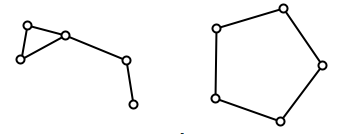
\includegraphics[scale=0.6]{equivalent}
\end{figure}

Ambos tienen 5 vértices, 5 aristas y número cromático 3. El primero tiene polinomio cromático $k(k-1)^3(k-2)$, lo cual se puede observar empezando a colorear por el vértice de grado 1. El segundo tiene polinomio cromático $(k-1)^5-(k-1)$ aplicando el cálculo de $P(C_n,k)$ del ejercicio \ref{ejer:3.6} para $n=5$, que es distinto del anterior.

%\url{https://math.stackexchange.com/questions/3024221/find-two-graphs-with-same-order-size-and-chromatic-number-but-with-different-c/3024250#3024250}
\end{solucion}

\end{document}
